\chapter{Simulation Experiments and Evaluation of the Architecture}
In this chapter, we present the results of simulation experiments developed to evaluate and explore choices offered by our K-HAS architecture. Using nodes with knowledge-processing capabilities to deliver interesting data quicker than a standard WSN, we have developed a simulation for our proposed architecture, K-HAS, as well as variations on the knowledge processing capabilities of the nodes at each tier.

The simulations were developed to determine whether K-HAS is the best mix of processing and collection nodes that maximises network lifetime while minimising the transmission time of interesting data. This was done by using a network structure, that matched our motivating scenario, and changing the knowledge-processing capabilities on each node at every tier; ranging from no knowledge on every node to the maximum knowledge-processing capabilities across the network. We aim to show that the more knowledge-processing capabilities that are pushed out towards the edge of the network, the more effective the network becomes at prioritising data that it believes to be interesting and delaying what it believes to be empty.

This chapter is structured as follows. Section \ref{sim:sim} describes the implementation of the network. Section \ref{sim:imp} outlines the results and Section \ref{sim:res} compares these with LORIS and the current solution in our motivating scenario. Section \ref{sim:conc} concludes our findings and highlights areas that require further experimentation.

\section{Simulation Environment}\label{sim:sim}

Using RePast Simphony \cite{Collier2003}, an agent-based network simulation tool developed in Java, we created a network to emulate K-HAS. RePast is an agent-based modelling system that allows for agents to be created and placed on a grid. Ticks denote a period of time and simulations can run for a fixed number of ticks, or until stopped. Ticks can also be used to schedule events, such as searching for neighbours, by calling methods that last for a set number of ticks, or begin at a particular tick. For example, a camera sensor node may be tasked with taking a picture every three hundred seconds. When the simulation reaches three hundred ticks (or six hundred, nine hundred, twelve hundred and so on), a scheduled event is run to simulate the camera's capture of an image and transmitting it to an endpoint.
%train may take three hundred for it to arrive at its destination. When the simulation reaches three hundred ticks, a scheduled event could run that would open the train doors, make an announcement and so on.

RePast was chosen because we did not require the low level network configuration provided by other tools, such as NS2 \cite{mccanne1997network}, but we did need to modify and record the behaviour between nodes as they capture and process sensed data. RePast's event scheduling allows for nodes to be modelled as agents and the dynamic configuration allowed us to modify the simulations during run time. The aim of these simulations was to visualise how different knowledge-processing capabilities can affect the prioritisation and transmission time of observations, as well as the accuracy of their classifications. RePast allowed us to utilise existing Java code we were using in our K-HAS middleware and develop a base simulation that could be configured easily with XML files.

Agents were created, using the RePast SDK, and Java classes were used to manipulate their behaviour. Simple networks may only contain basic agents with only a few variations from those provided by RePast. However, for more complex networks, a hierarchy of agents is required and Java's inheritance can then be used to create subclasses of an agent.

A 2D space is used to display the grid and the simulation is run within RePast's own GUI. This GUI provides functionality such as editing the properties of classes, integrating with Matlab, taking screenshots and saving different configurations of the same network.


\section{Experiment Design}\label{sim:imp}
	While the aim of these simulations was to show the effectiveness of K-HAS over the current solution, we also wanted to determine if it was the optimal solution, in terms of delivery of interesting data and network lifetime. We believe that the ideal solution would be to attach nodes with high knowledge-processing capabilities to all cameras in the network, however the short battery life means that replacements would be made as often as the current manual solution, detailed in Section \ref{tech:motiv}.

	Throughout this chapter, we will be referring to nodes tasked with different purposes as the three definitions listed here:
	\begin{itemize}
		\item Sensing Node: A node that has been tasked with the captuing, and routing, of sensed data.
		\item Routing Node: A gateway node that is tasked with collecting, processing and forwarding sensed data.
		\item Central Node: A node with similar functionality to a typical base station, tasked with storing all sensed data and providing an interface to users.
	\end{itemize}

	At the routing and sensing tier, the degree of knowledge processing capabilities can range from the levels outlined below:
	
	\begin{itemize}
		\item No Knowledge (NK): The node possesses no knowledge processing capabilities.
		\item Minimal knowledge (MK): The node possesses basic knowledge processing capabilities and contains a static rule base (Section \ref{khas:dc}).
		\item High Knowledge (HK): The node possesses high knowledge processing capabilities and is able to process data, metadata and use a dynamic rule base (Section \ref{khas:dp}).
	\end{itemize}
	
	The higher knowledge-processing capabilities of HK nodes allow them to classify observations with a greater accuracy, but their battery life is much shorter than MK nodes due to their increased power needs (Section \ref{tech:hw}). In contrast, MK nodes can run for a longer period without requiring battery replacement. MK nodes, however, are unable to classify observations to the same level as HK nodes. While HK nodes can classify an observation as interesting or empty and, in our scenario, match to a species, MK nodes can only assume an observation is interesting using the image's metadata as they lack the capabilities to reliably determine whether an observation is empty or not. The scenarios we have implemented cover combinations of HK, MK and NK, in a twenty five node network. We use twenty five nodes because DGFC had a between twenty and twenty two active cameras during our first and second visits and we knew that the first implementation of the network would require a single endpoint. From this, we chose to use four routing nodes so that each could handle an equal number of sensing nodes, if they were all within range, and a single central node. Our experiments in Danau Girang were restricted to a smaller number of nodes, due to cost, but we expected to deploy a sensing node onto all of the active cameras. The hierarchical nature of the network is shown in Figure \ref{fig:sim} and explained later in this section. These scenarios were developed to determine which combination of MK, NK and HK nodes allowed for the greatest accuracy when delivering interesting sensed data. As a benchmark, we have also included scenarios that simulate a standard WSN where nodes have no knowledge asnd simply forward to a base station with knowledge processing capabilites, these scenarios have been outlined below:
	
	\begin{itemize}
		\item NK-NK-NK: All nodes possess no knowledge processing capabilities.
		\item MK-MK-NK: Sensing and routing nodes possess minimal knowledge processing capabilities.
		\item NK-MK-NK: Sensing nodes possess no knowledge processing and routing nodes have minimal knowledge.
		\item MK-HK-NK (K-HAS): Sensing nodes have minimal knowledge and routing nodes possess high knowledge. This scenario matches the K-HAS architecture we proposed in Chapter \ref{chap:arch}.
		\item HK-HK-NK: Sensing and routing nodes have high processing capabilities.
		\item NK-NK-MK: Sensing and routing nodes have no processing capabilities and central nodes have minimial knowledge processing capabilities.
		\item NK-NK-HK: Sensing and routing nodes have no processing capabilities and central nodes have high knowledge processing capabilities.
	\end{itemize}


In the final two scenarios, routing nodes are not used and sensing nodes connect directly to the central node as their purpose would only be for routing and the range of Zigbee allows sensing nodes to be within range of the central node.

Before implementing, we designed the agents required based on the nodes described in the ontology we proposed in Chapter \ref{chap:ont}. Using that, we created a hierarchy of nodes inheriting common properties from a node object. As previously mentioned, we had metrics on range and transmission times from previous experiments and the deployment of LORIS. We used these to create properties for each transmission medium that could be used by each node object. Table \ref{sim:tab:terms} shows how the K-HAS terms, introduced in Chapter \ref{chap:arch}, and LORIS terms, detailed in Chapter \ref{chap:imp}, map to the node types described above. The nodes used in our simulations map directly to the ontology.

\begin{table}[h]
\centering
\begin{tabular}{|l|l|l|}
\hline
\textbf{Network Type} & \textbf{Original Term} & \textbf{Maps To}          \\
\hline
K-HAS                 & DC Node                & Sensing Node + MK         \\
                      & DP Node                & Routing Node + HK         \\
                      & DA Node                & Central Node + HK         \\
LORIS                 & Buckeye                & Sensing Node + NK         \\
                      & DA and DP              & Routing/Central Node + HK \\
\hline
\end{tabular}
\caption{Mapping of K-HAS to Simulation Terminology}
\label{sim:tab:terms}
\end{table}

Using a Java library we developed for DwC archives during the implementation of LORIS (Section \ref{loris:arch}), we were able to implement DwC archives as the data standard in our simulations, this allowed us to model the prioritisation of sensed data, as well as the classification of observations, in the same way that a K-HAS deployment would.

The structure of the simulation is as follows: The \textit{network builder} instantiates all the nodes, places them randomly on the grid and schedules events once the simulation has started. The nodes then use the properties of their transmission medium to find nodes in range and create a connection; depicted by a line between the node. The simulation uses metrics, such as the size of the image, extracted from the images taken at Danau Girang and the chance of an image being captured by a camera is based on the average capture rate of a camera. The fire rate has been calculated by the average number of pictures captured in a day taken by each camera. Figure \ref{fig:sim} shows an example topology of the MK-HK scenario, sensing nodes are marked in yellow, routing nodes in green and the central node is red. Black edges are used to link the nodes. Each node is placed randmonly on the space and links are established between neighbouring nodes with the fewest hops to a central node. Network parameters are set in a configuration file, before the simulation runs, such as: the number of each node type and the size of the space.


	\begin{figure}[h]
	\centering
	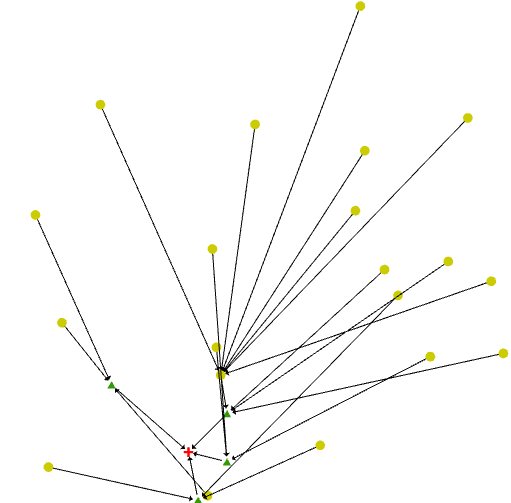
\includegraphics[width=0.8\textwidth]{Chap7/figures/khas_sim}
	\caption{MK-HK Simulation Example in RePast Simulator}
	\label{fig:sim}
	\end{figure}


\subsection{Darwin Core}\label{sims:exp:dwc}
The Darwin Core class represents a DwC archive, encapsulating \textit{Identification}, \textit{Location}, \textit{Occurrence}, \textit{Image} and \textit{Species} (Section \ref{buildcapture}). The images we have collected from Danau Girang were processed to find details such as the average size when captured at night and day, how often an average camera triggers and the percentage of images with animal content. These data were then used to specify how often a randomly placed node should capture an observation per tick.

Upon each capture, images are created and given a random size, between the maximum and minimum size found in the 120,000 images collected from DG. The sum of the image sizes is used to calculate the size of the archive. Using this size, a sensing node calculates how long the archive takes to send based on the size and the transmission rate. We assume that the rate stays constant for the duration of transmission.
When an archive is sent to the routing node, we used the average time for our image processing tool and Drools engine to run and attempt a classification, which is 43 seconds (ticks), explained in detail in Section \ref{tech:sf:triton}. To keep the classifications as general as possible, so that the simulation applies to any WSN for scientific observations, archives are not classified down to the species level, they are marked as \textit{interesting} or \textit{empty} and then forwarded to the central node.

\subsection{Routing}
The routing protocol used needs to be dynamic in order to adapt to nodes being added and removed during deployment, while minimising traffic in a resource constrained network. In our approach, we use a modification of the Minimum Cost Forwarding Algorithm (MCFA), described in Section \ref{arch:routing}. A cost is assigned to each node, based on how far they are from the central node, with neighbouring nodes choosing to connect to the node with the lowest cost. However, in normal implementations of MCFA, all nodes are of the same type and simply need to connect to a central node. This protocol is used in all scenarios.

In our K-HAS architecture, sensing nodes cannot connect directly to a central node because processing would not take place. Because of this, we used the same routing method across all scenarios. Our implementation of MCFA works with a discovery phase and a transmission phase. The discovery phase is a scheduled event, taking place at the start of deployment but it can be run throughout deployment to react to nodes being added or removed. 

\subsubsection{Discovery}\label{sim:disc}
	Discovery begins at each central node, scanning nodes in range for routing nodes and sending a broadcast packet, with a cost of 0, to inform them that they are within range of a central node. Links between Central and Routing nodes use W-Fi in all of our scenarios. Once received, routing nodes increment the count and forward the packet to any routing nodes within range of them, where we use the range of Zigbee. We found that this method overloaded the routing nodes and all sensing nodes within range would connect to the first routing node they receive the broadcast from. We then implemented a method, called \textit{load balancing} \cite{Gupta2003}, which uses the sensing nodes connected to a routing node to calculate whether it should offload new nodes to a neighbouring routing node.
	
	The maximum connections a routing node can have is determined by the total number of sensing nodes in the network divided by the total number of routing nodes, which is held in the knowledge base of the central node. Once a routing node has the maximum number of connections allowed, it starts to offload to a neighbouring routing node that is also in range of the sensing node requesting a connection. If there are no neighbouring nodes then the routing node exceeds the maximum number of connections allowed, to save sensing nodes being left with nowhere to send their data.
	
	If the sensing node that receives the broadcast does not have an existing route to a central node, or the cost of the current route is higher than the received route, it adds an edge to the routing node, increments the count and forwards it to all nodes in range. This process continues until the broadcast reaches the edge of the network. Nodes do not have global knowledge of the route to the central node, only of their neighbour with the lowest cost.
	
	This phase can be repeated throughout the course of the deployment, simply by scheduling it as an event to occur every \textit{n} ticks. However, the simulation currently only uses the discovery phase at the beginning of the deployment.
	
\subsubsection{Transmission}
	Once the discovery phase has been completed, providing nodes are within range of the central node, the transmission phase begins where only DwC archives are then sent across the network. Observations are captured based on the mode of the simulation and sent to the lowest cost neighbour.
	
	In order to manage transmissions, sensing nodes have a \textit{SendState} object that contains the next archive to send, the time to send it and whether it is currently sending. This is used to determine what operations to perform, once an archive has been sent, it is deleted from the SendState and the sending flag is set to false. A new archive is then added and sent when the opportunity arises.
	
	When a routing node receives the archive, it begins processing. Routing nodes use the SendState as well, but they only add an archive once it has been processed and they then select the oldest archive that has been classified as interesting, providing an archive is not already waiting to be sent. The archive stores information about the route it takes, recording every hop, as well as the time it took from capture to central node.
	
	Scheduled sending events run every thousand ticks, which is configurable, to check the sending state of the node and send any archives in the SendState. The node then waits for the number of ticks that it will take in order to transmit the archive.
	
	Once the simulation is completed, either manually or through a defined number of ticks, all captured observations are iterated over and written to a CSV file, with details such as the path it took (if delivered), total transmission time, content and time of capture.
	
\subsection{Capture}\label{sims:exp:cap}
	Using the existing data collected from Danau Girang, we calculated how often a camera triggers in a six month deployment, as well as how often the observation contained interesting content. 
	
	To calculate the count of interesting images, we processed every directory of images to extract the largest object in the foreground, using our Triton program. Once processed, we iterated through every directory, counted the total number of images and the total number of extracted images; an extracted image is a black and white image containing the largest object that has been found in the observation and are only created when the processing believes that the observation is interesting. This gave us a 20.7\% chance of an image being interesting, across every camera.
	
	The chance of a camera being triggered each second was calculated by the total number of observations (13,399) divided by the number of seconds in six months (15,552,000). This gives a chance of 0.000861561 of a camera trigger in any given second.
	
\subsection{Processing}
	The types of knowledge processing capabilities that we outlined in Section \ref{sim:imp} are used in the simulation to determine which type of processing to perform on observations. The result of processing is that an observation is marked as interesting or empty. The limitation of our image processing tool is that only the largest region of interest (ROI) is extracted, even if there are multiple objects in the image. The outcome can be any of the following:
		\begin{description}
			\item True positive (TP): An ROI is extracted that contains the animal in the set.
			\item False positive (FN): An ROI is extracted that contains nothing of interest.
			\item True negative (TN): A camera is triggered with nothing of interest in the image and no ROI is extracted.
			\item False negative (FN): An image containing an animal has no ROI extracted.
		\end{description}
	
	Using the results of our image processing application (explained in Section \ref{tech:sf:triton}) for the properties of HK processing, we encoded that an 82\% accuracy at detecting TP images, with a 98\% accuracy for finding TN images. Nodes with MK do not have the ability to mark an image as empty, but they can mark an image as interesting. However, the results we have from our rule base are not as extensive as the results we have for Triton (due to limited local knowledge and existing rules approved by domain experts), so instead we use a predefined 10\% accuracy for detecting TPs. This 10\% is used because we needed to show the difference between a node with MK and a node with HK. HK nodes have the ability to process the contents and metadata of sensed data, with access to libraries and a dynamic knowledge base. MK nodes are able to look at the basic metadata and only have a static knowledge base, limited in size. In future work, we could test with greater accuracy or, with more rules, we could run experiments to find the exact accuracy of an MK node. An interesting image is an image that contains an animal and can be either a TP or FN. Empty images are those that do not contain an animal and can be either FP or TN.

	We assume that central nodes do not have the power limitations of nodes deployed in the field and have the ability to have more compuational power, so they are able to process up to four observations simultaneously and the processing time is only 30 ticks for HK capabilities, while MK remains at 5 ticks. An observation is not marked as delivered unless it has been processed by the central node.

\subsection{Simulation Configuration}
	Simulations in Repast are configured through XML files and read in, by Java classes, as parameters. It is this parameters file that allows one to set the number of nodes in the space, the size of the space, knowledge levels of nodes, bandwidth availability or the chance of image capture or the chance of an image containing something of interest, an example of this file can be seen in Appendix \ref{appendix:sims:params}.

	Section \ref{sims:exp:cap} explains how we calculate the chance of an interesting image and the chance of capture at any given tick. The file size of images in each observation is randomly calculated between an upper and lower bound found in the images collected from Danau Girang (Section \ref{sims:exp:dwc}) and the transmission rate is either fixed at the maximum rate or based on a random number between twenty and the maximum; this is determined by the mode set in the parameters file (ideal or variable). In order to saturate the network, we multiplied the chance of an image being captured by 10.


	

\section{Results}\label{sim:res}

In this section, we analyse the results of each scenario and their variations to compare the delivery of interesting data versus empty data for all the network scenarios outlined in Section \ref{sim:imp}. Each scenario was run 50 times with four variations:
\begin{description}
	\item Normal bandwidth availability with ideal transmission rate.
	\item Normal bandwidth availability with variable transmission rate.
	\item Saturated bandwidth availability with ideal transmission rate.
	\item Saturated bandwidth availability with variable transmission rate.
\end{description}

\subsection{Normal Network Saturation with Ideal Transmission Rate}

With normal saturation, almost all data was delivered in the duration, with HK-HK-NK and MK-HK-NK delivering around 99\percentage and NK-NK-MK and NK-NK-HK delivering less, most likely due to the build up observations at the central node, with only a single node processing.

	\begin{figure}[h]
	\centering
	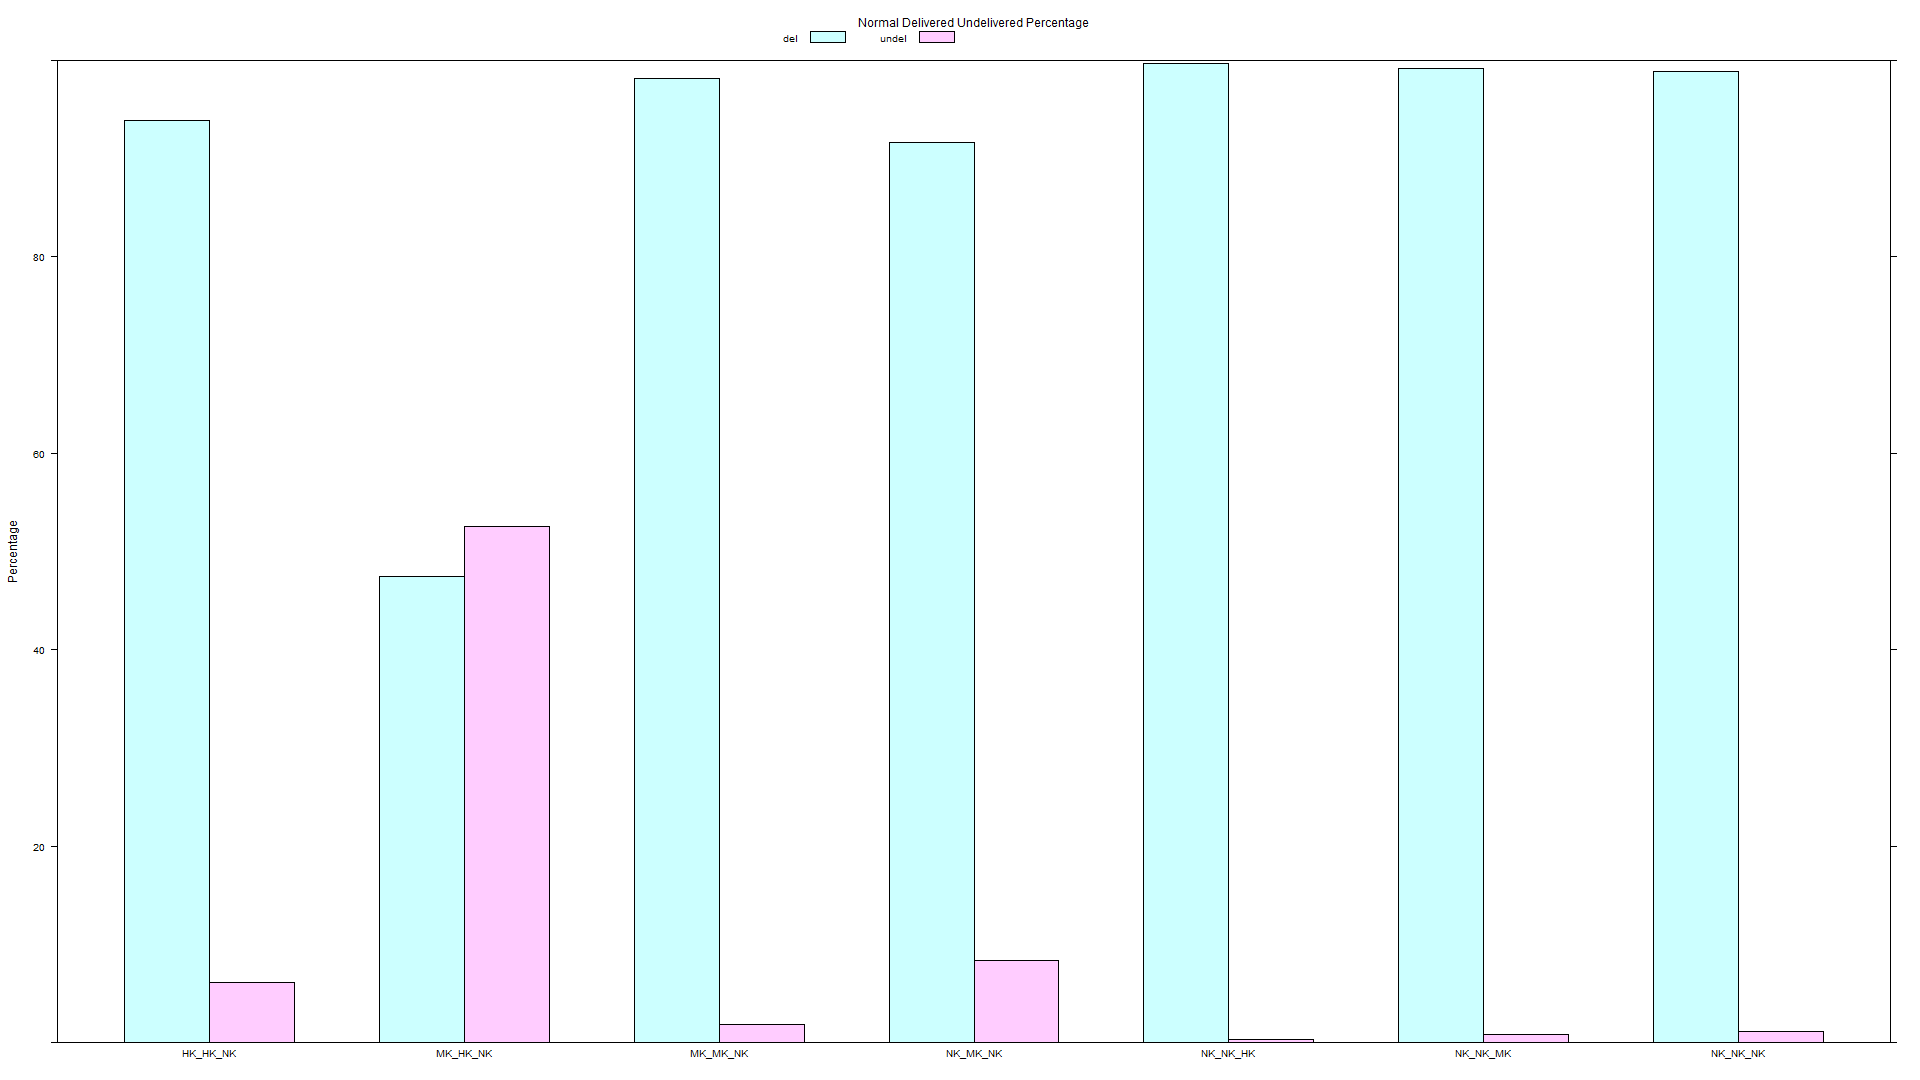
\includegraphics[width=0.8\textwidth]{Chap7/figures/plots/normal_ideal/delvsundel_percent.png}
	\caption{Delivered vs Undelivered Observations for Normal Saturation and Ideal Transmission Rate}
	\label{fig:sim:res:norm:ideal:delundel}
	\end{figure}

	Figure \ref{fig:sim:res:norm:ideal:tpfp} shows that the delivery time for interesting observations can decrease with higher knowledge processing capabilities towards the edge of the network, but even pushing minimal knowledge processing capabilities to the edge reduces the transmission time significantly. However, the faster delivery time of \textit{true positives} with MK-MK-NK is most likely due to the lower chance of an image being classified correctly, so there are fewer observations to average. Comparing this with \ref{fig:sim:res:norm:ideal:tnfn}, we can see that there is a noticeable difference between interesting and empty observations but it is not large, mainly due to the fact that the network almost always had available bandwidth, so prioritisation was not key, this is evidenced by Figure \ref{fig:sim:res:norm:ideal:intempt} which shows that the split of interesting and empty images delivered matches the 20.7\percentage chance of an interesting image being captured.

	\begin{figure}[h]
	\centering
	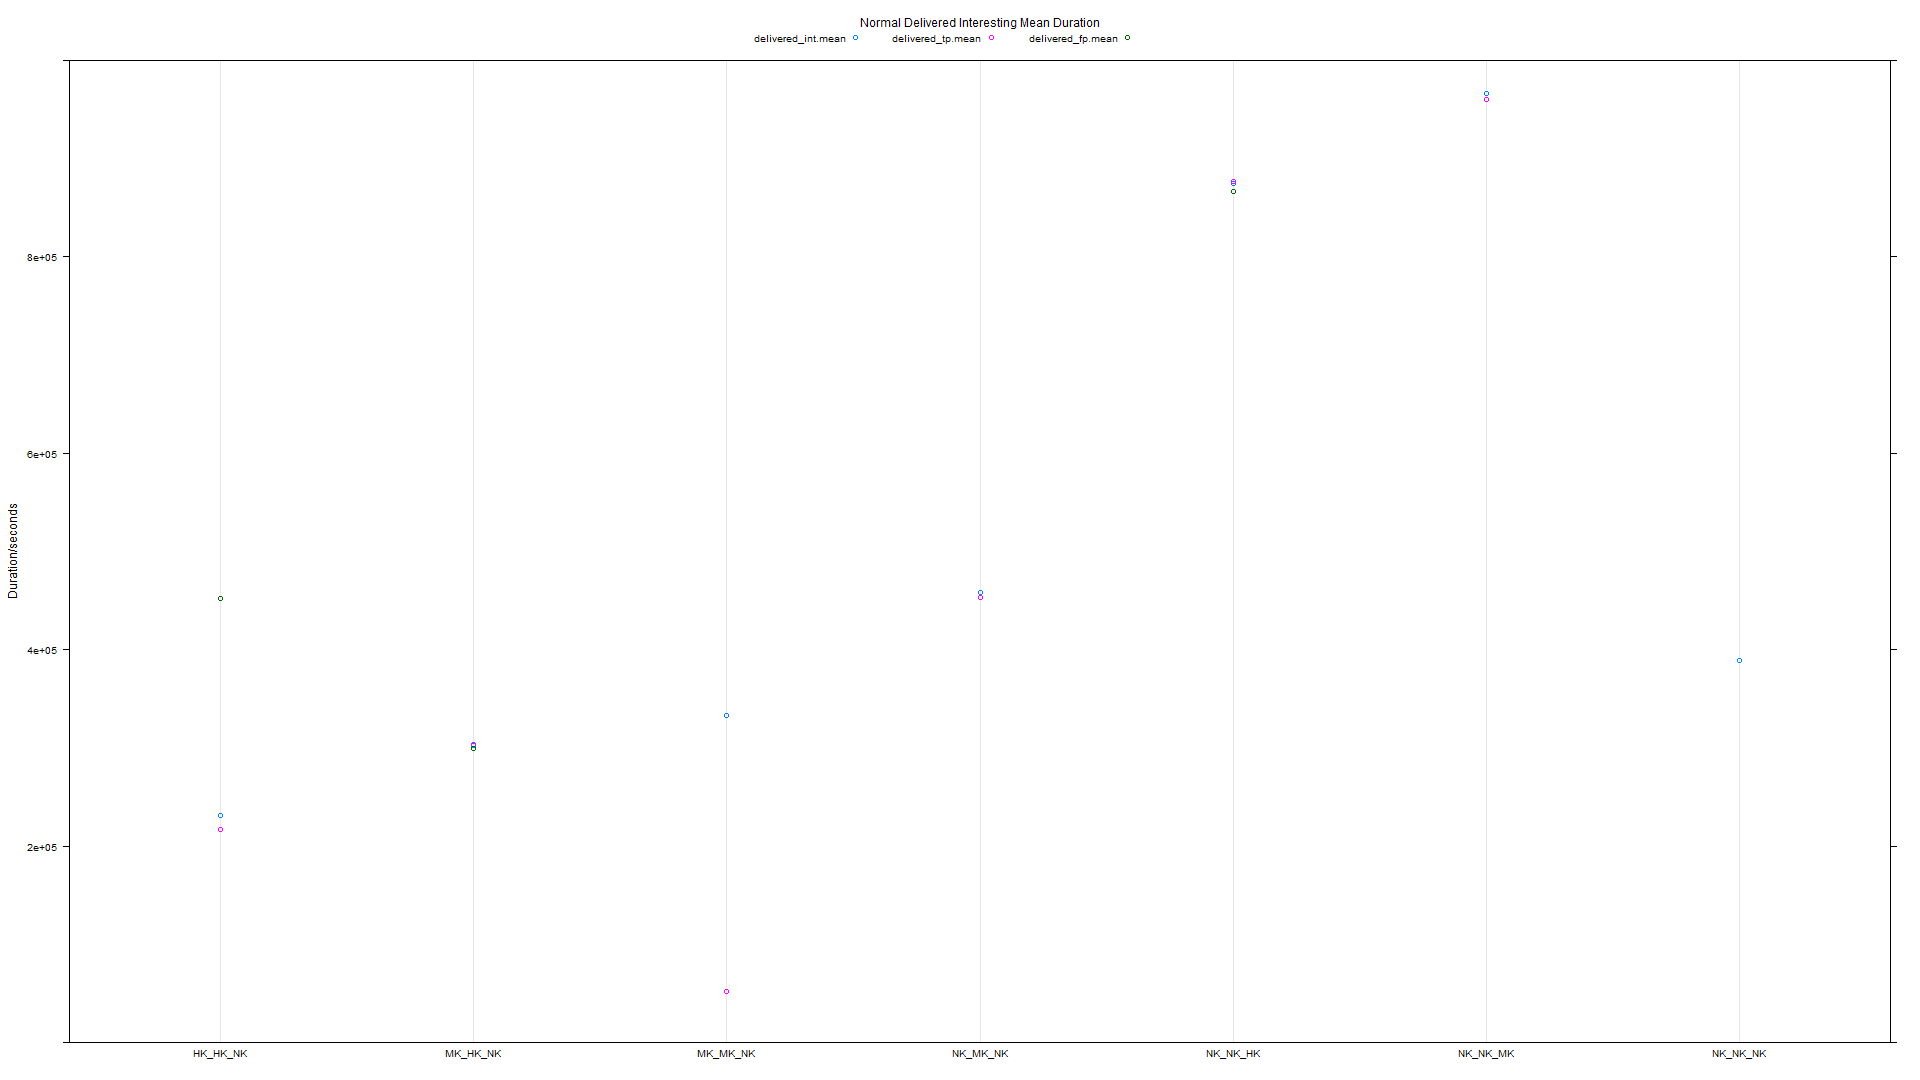
\includegraphics[width=0.8\textwidth]{Chap7/figures/plots/normal_ideal/tpvsfp_delivered.png}
	\caption{Average Delivery Time for Interesting Observations with No Saturation and Ideal Transmission Rate}
	\label{fig:sim:res:norm:ideal:tpfp}
	\end{figure}

	\begin{figure}[h]
	\centering
	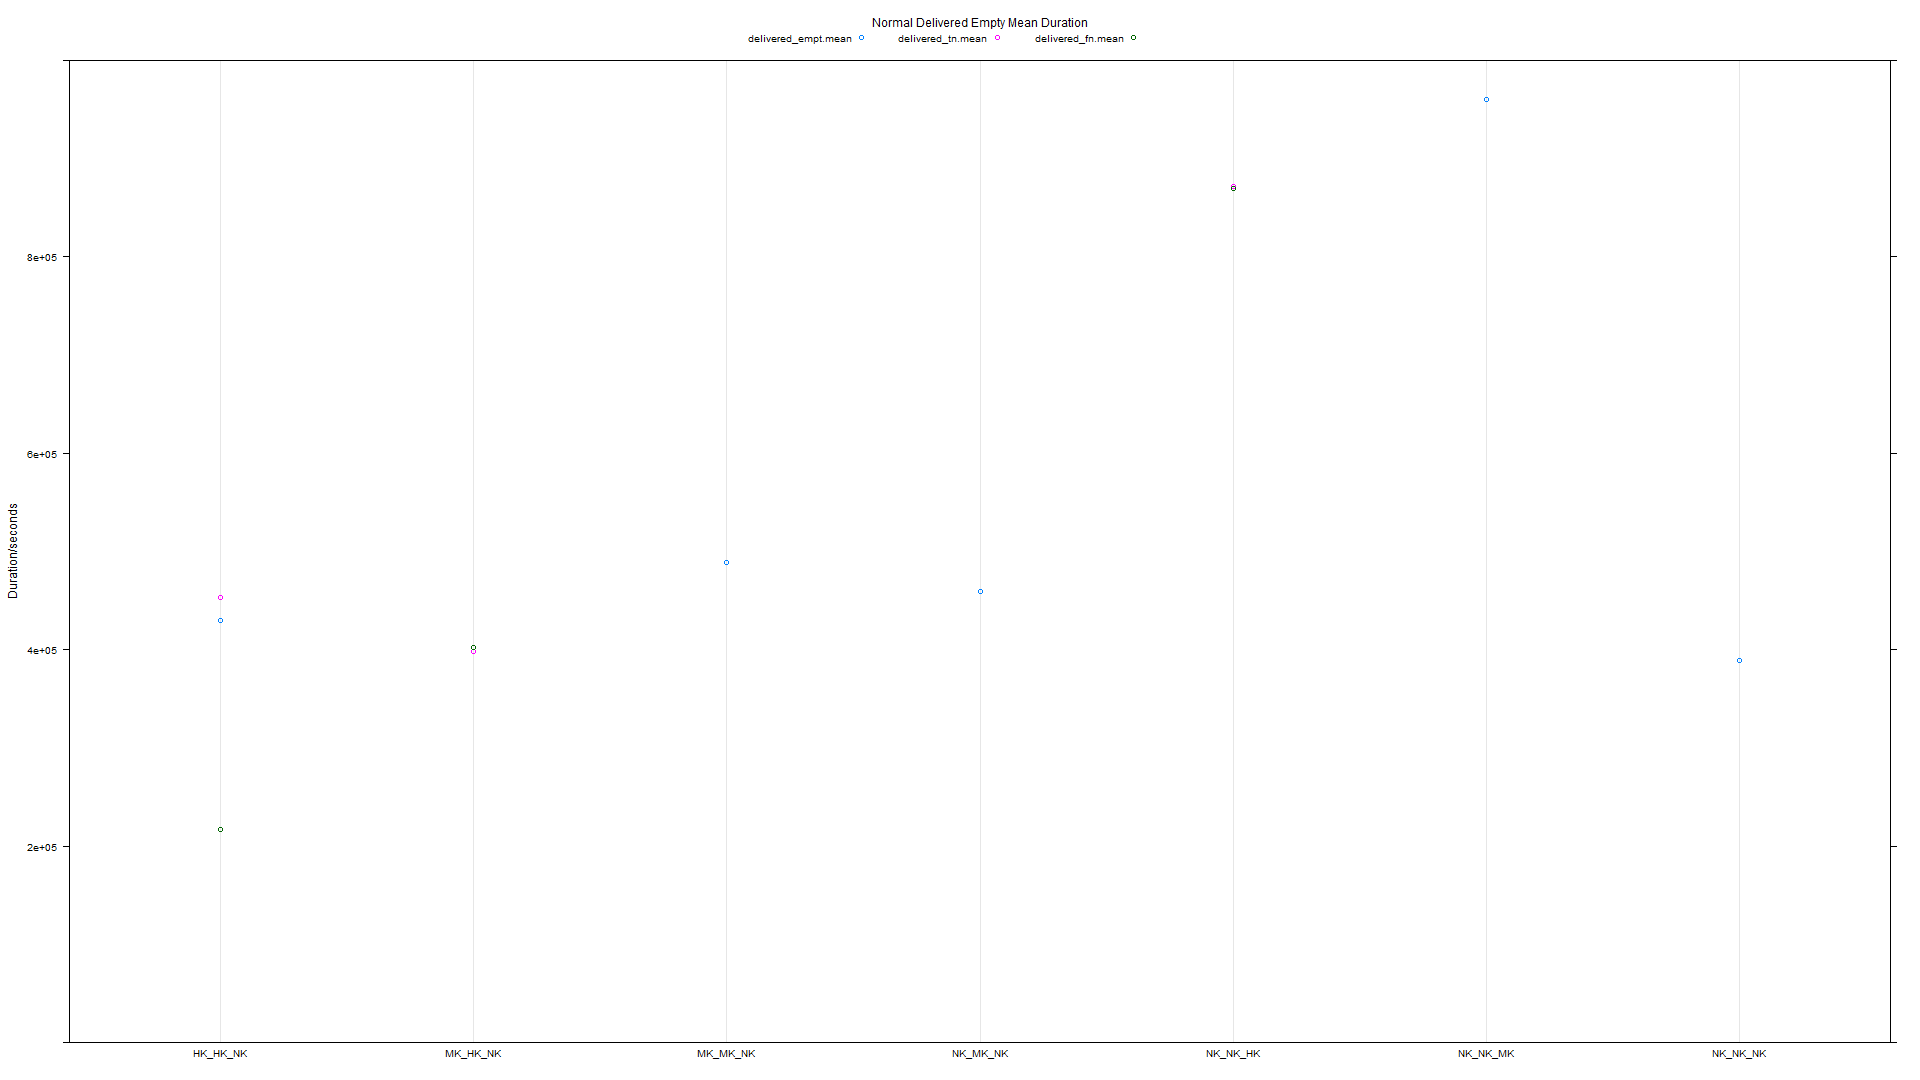
\includegraphics[width=0.8\textwidth]{Chap7/figures/plots/normal_ideal/tnvsfn_delivered.png}
	\caption{Average Delivery Time for Interesting Observations with No Saturation and Ideal Transmission Rate}
	\label{fig:sim:res:norm:ideal:tnfn}
	\end{figure}

	\begin{figure}[h]
	\centering
	\includegraphics[width=0.8\textwidth]{Chap7/figures/plots/normal_ideal/intdelvsempydel_percent.png}
	\caption{Interesting vs Empty Delivered Observations with No Saturation and Ideal Transmission Rate}
	\label{fig:sim:res:norm:ideal:intempt}
	\end{figure}



\subsection{Normal Network Saturation with Variable Transmission Rate}

\subsection{Saturated Network Saturation with Ideal Transmission Rate}

When the chance of an image being captured is increased tenfold then the network architecture must use the knowledge processing within the network to prioritise those that have been classified as interesting. Figure \ref{fig:sim:res:saturated:ideal:delundel} shows that a network with no knowledge processing delivers a higher percentage of observations and that the percentage delivered reduces when knowledge processing capabilities are pushed further towards the edge.

	\begin{figure}[h]
	\centering
	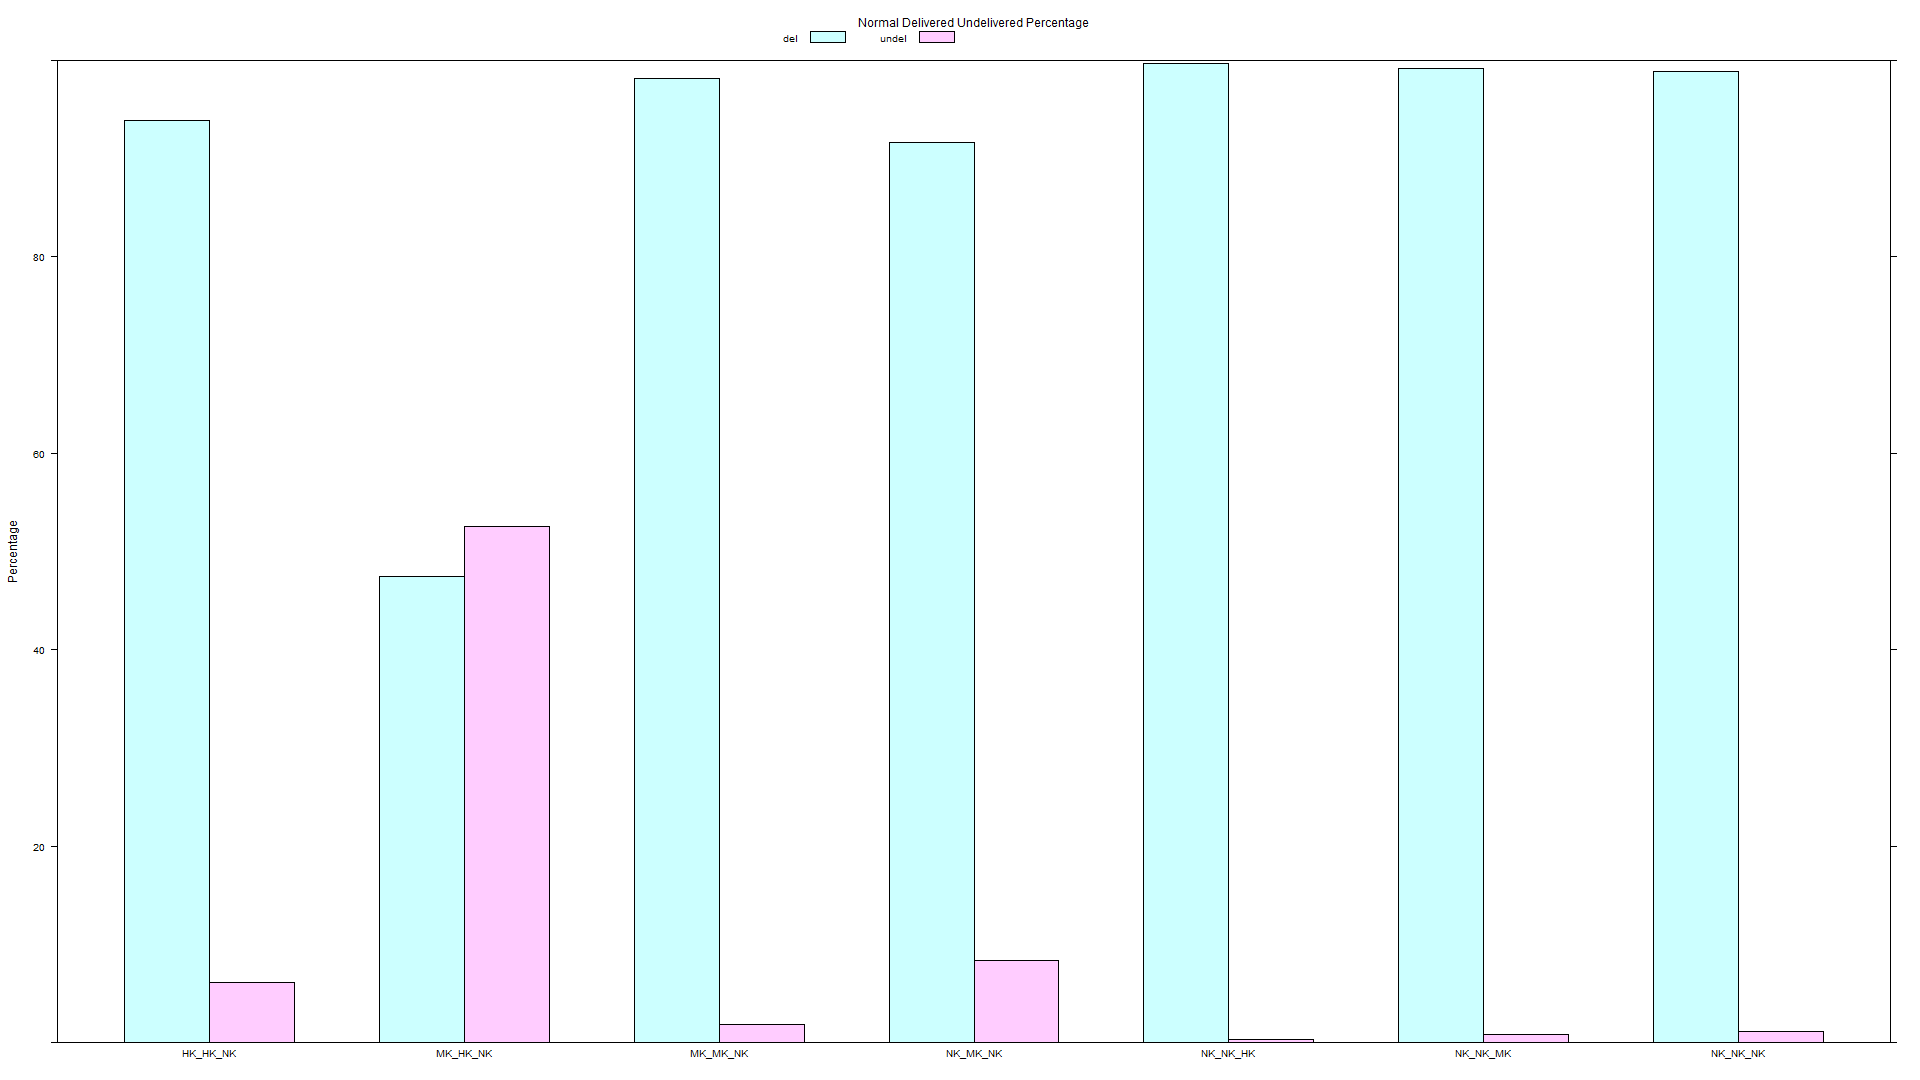
\includegraphics[width=0.8\textwidth]{Chap7/figures/plots/normal_ideal/delvsundel_percent.png}
	\caption{Delivered vs Undelivered Observations for Normal Saturation and Ideal Transmission Rate}
	\label{fig:sim:res:saturated:ideal:delundel}
	\end{figure}

	Figures \ref{fig:sim:res:saturated:ideal:tpfp} and \ref{fig:sim:res:saturated:ideal:tnfn} highlight that higher knowledge processing capabilities significantly reduce the delivery time for interesting observation the further out into the network the capabilities are pushed and the higher the knowledge capabilities, the greater the number of \textit{true positives}. HK-HK-HK allows for prioritising straight from the edge of the network and routing nodes merely act as forwarding nodes to the central node whereas MK-HK-NK allows for some prioritisation at the edge and the routing nodes can then use their HK capabilities. Only having processing power at the centre of the network means that no prioritisation can occur and the central node acts as a bottle neck; a bottle neck that could be alleviated by adding more processing power or even more central nodes, admittedly.

	\begin{figure}[h]
	\centering
	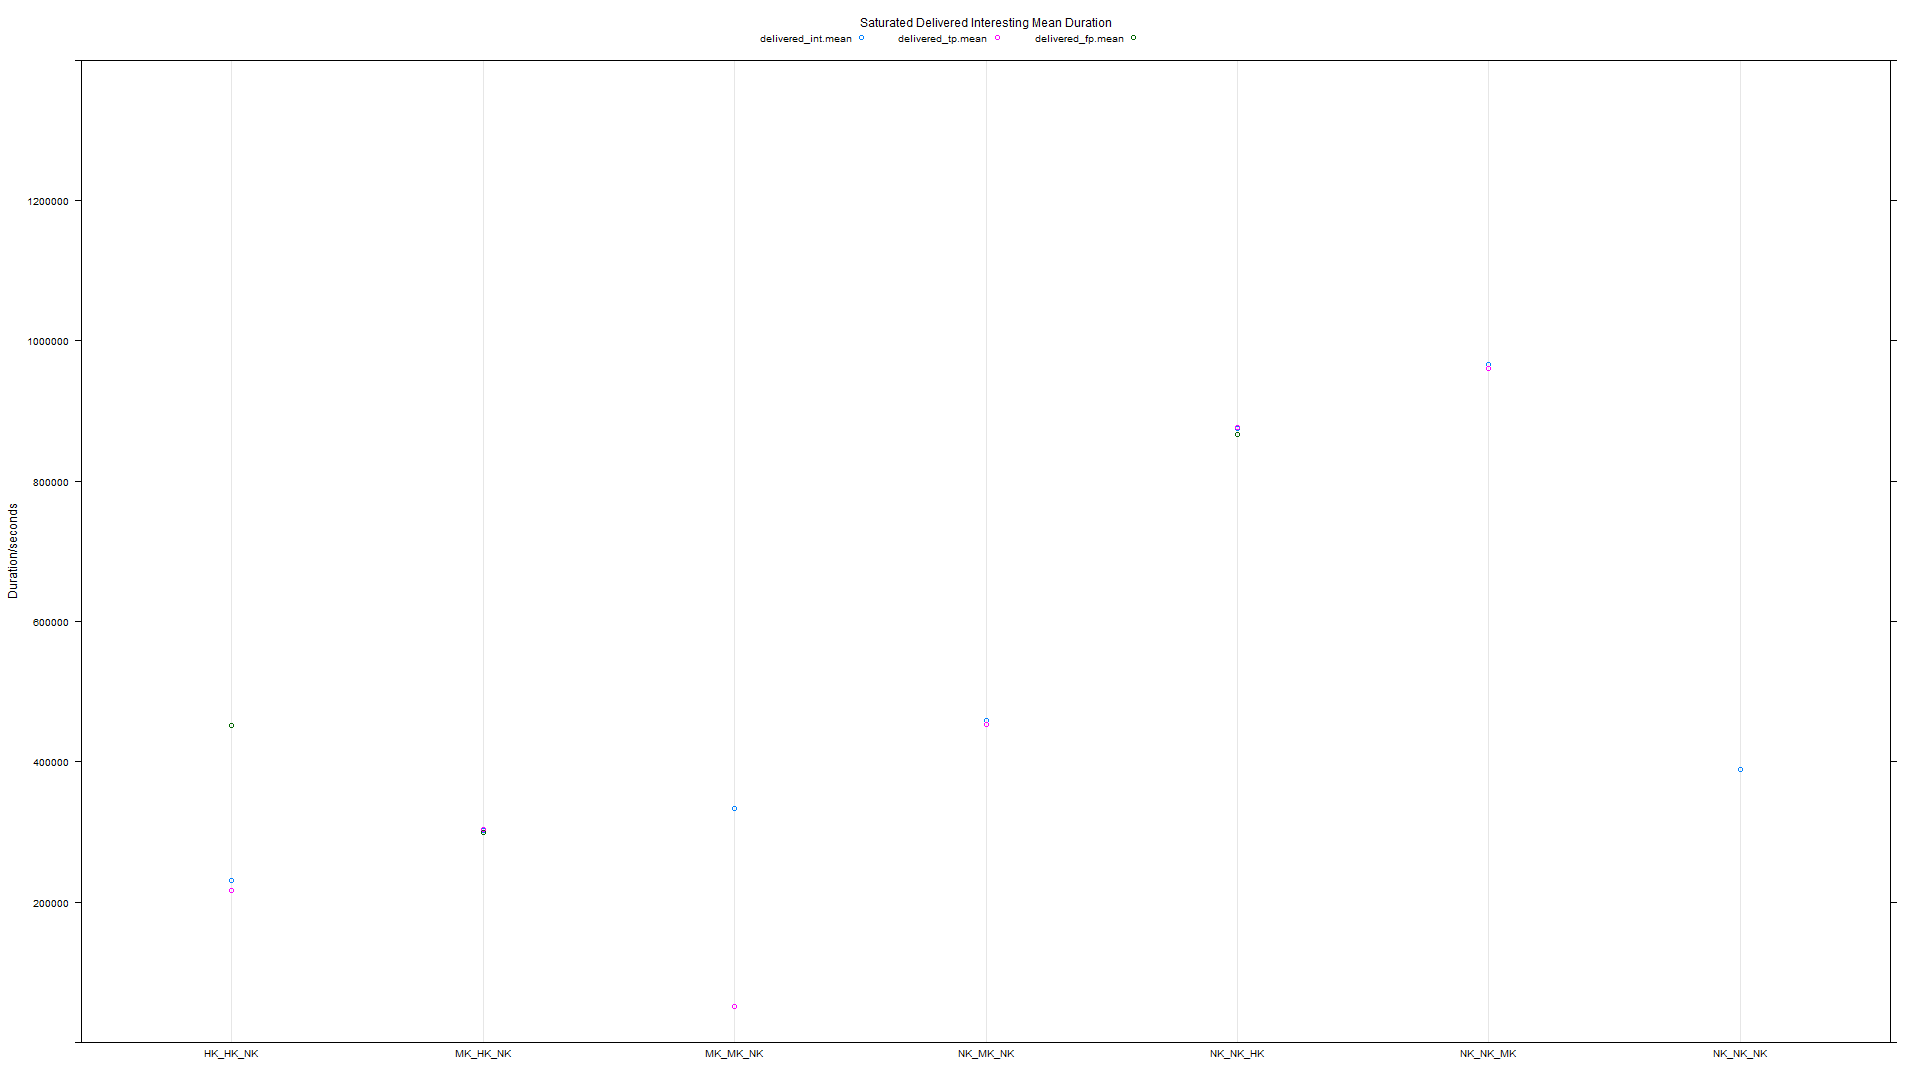
\includegraphics[width=0.8\textwidth]{Chap7/figures/plots/saturated_ideal/tpvsfp_delivered.png}
	\caption{Average Delivery Time for Interesting Observations with Saturation and Ideal Transmission Rate}
	\label{fig:sim:res:saturated:ideal:tpfp}
	\end{figure}

	\begin{figure}[h]
	\centering
	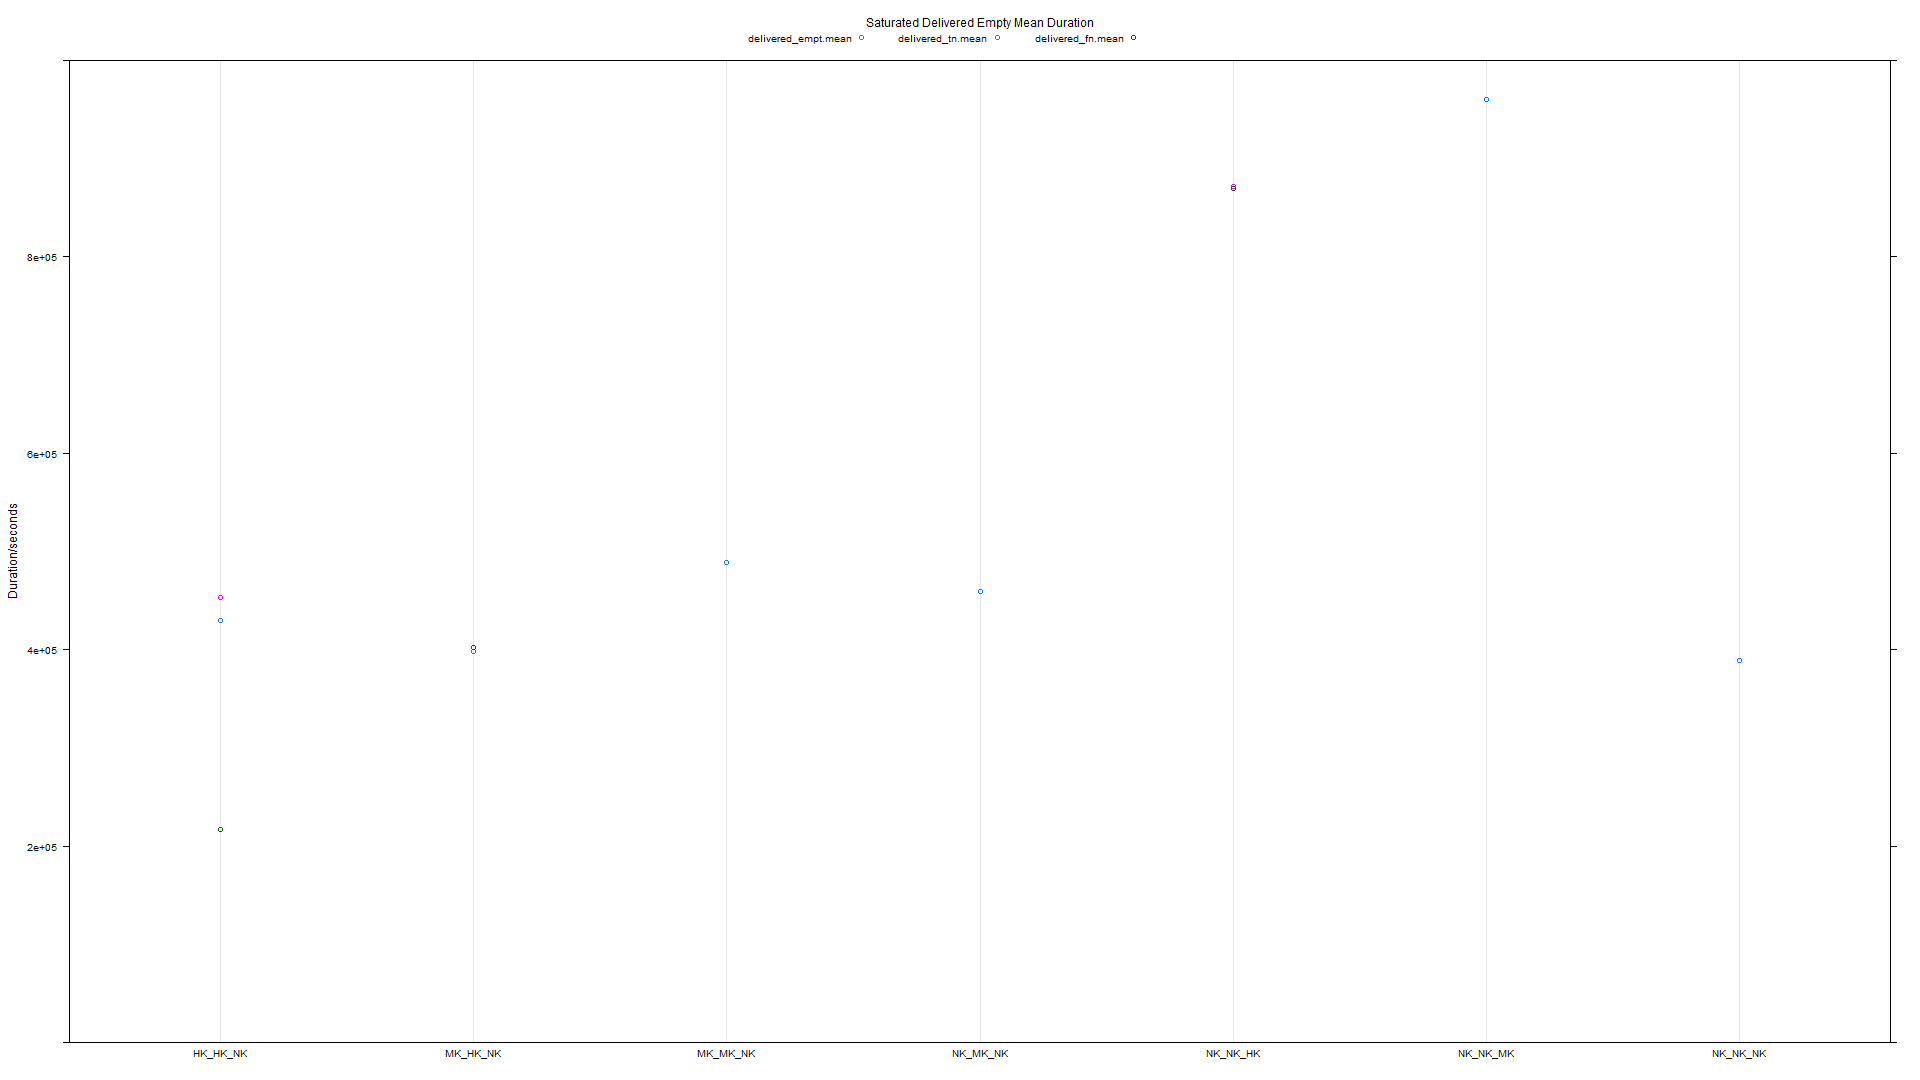
\includegraphics[width=0.8\textwidth]{Chap7/figures/plots/saturated_ideal/tnvsfn_delivered.png}
	\caption{Average Delivery Time for Interesting Observations with Saturation and Ideal Transmission Rate}
	\label{fig:sim:res:saturated:ideal:tnfn}
	\end{figure}

	Figure \ref{fig:sim:res:saturated:ideal:intempt} shows the percentage of interesting and empty observations delivered of all the observations captured. As is expected, NK-NK-NK has the largest number of total observations delivered and processing at the central node only reduces the number of deliveries. It should be noted, however, that the central node may hold more observations that have not been processed and thus not marked as delivered. HK-HK-HK's ability to prioritise from the edge provides a decent proportion of interesting observations compared to the others but comes with the cost of using nodes that are less power efficient and we can see that MK-HK-NK and Mk-MK-NK are a good trade off that could increase the network lifetime.

	\begin{figure}[h]
	\centering
	\includegraphics[width=0.8\textwidth]{Chap7/figures/plots/saturated_ideal/intdelvsempydel_percent.png}
	\caption{Interesting vs Empty Delivered Observations with Saturation and Ideal Transmission Rate}
	\label{fig:sim:res:saturated:ideal:intempt}
	\end{figure}

\subsection{Saturated Network Saturation with Variable Transmission Rate}


\section{Conclusion} \label{sim:conc}
	







































